\chapter{Conclusion}
The goal of this thesis was to explore the capacity of different GIRG model variants to match a dataset of real social network graphs, due to their suspected inherent geometrical generation and power law tailed degree distribution. We pursued this in two relatively distinct efforts:
\begin{enumerate}
    \item using the high level framework of \cite{blasius2018towards} in \cref{chap:GGM} to assess realism of different generative models on various global graph statistics
    \item exploring methods to fit GIRG node weights and locations for an input real graph in \cref{chap:diff_maps} and \cref{chap:likelihood_point_estimation}
\end{enumerate}
There was also a third effort, to use graph kernels as an alternative to Bl{\"a}sius's framework for evaluating a generative model's realism, which was unsuccessful, and documented in \cref{chap:graph_kernels}.

1. showed GIRGs to perform similarly or better in realism than other simpler generative models, with different types of GIRGs excelling in simulating different  statistics of the real graphs. 2. showed more concretely that GIRGs are expressive enough to replicate the connectivity of these social networks. Both 1. and 2. showed that $d > 1$ dimensional GIRGs generally did not improve significantly on 1d GIRGs, but suggested that higher dimensions might work best in a mixed min/max GIRG or distorted GIRG framework where there's a natural downwards progression of influence of dimensions.


% In documenting our various experiments, we also detailed our methods and ideas for working with GIRGs and graph data which may prove useful to other practitioners.

% Our first achievement was to follow the realism framework of \cite{blasius2018towards}, to compare a range of generative graph models, including many GIRG subtypes, in their ability to replicate global statistics of a set of 104 social network graphs.
% Our results showed that GIRGs showed superior performance in replicating several key statistics: node closeness centralities, node betweenness centralities, effective graph diameter, and mean local clustering coefficient. We identified variations between different GIRG subtypes, with max norm cube GIRGs excelling at diameter replication, MCD GIRGs on closeness centrality, and max norm torus GIRGs on betweenness centrality. 
% Interestingly, increasing the geometric dimension did not yield significant improvements, indicating that 1-3 dimensions might be adequate to achieve a high-level similarity to real-world graphs. 1d often proved best, however mixed min/max GIRGs demonstrated good performance while having higher dimensionality, they should be explored further along with distorted GIRGs.

% Subsequently, we explored fitting GIRG node geometric location parameters to real-world social network graphs, to see if GIRGs are capable of exact replication of them on a node and edge level. This proved quite successful, showing that GIRGs can capture a high percentage of edges, even with just 1 dimension. Adding further dimensions is computationally intensive and doesn't increase the fit substantially. Our range of fitting methods might be further refined in practice according to the use case. 

\paragraph{Future Work}
The different GIRG variants that we have covered have only recently risen to prominence, and future work might compare them more thoroughly, both practically in relation to real graphs and theoretically.
% In particular, the mixed min/max GIRGs and distorted GIRGs are promising.
Other real graph datasets than the Facebook social networks we used might be explored, particularly ones where ground truth node attributes are known. These might provide a geometric influence on edges, and be compared to fit GIRG node locations.
% Whether they can be well fit by GIRGs using methods similar to ours would be fascinating.
Adapting the GIRG uniform location priors and power law weight priors to something more flexible and realistic to real-world data could also be fruitful.


\paragraph{Many thanks} to my supervisors Marc Kaufmann and Ulysse Schaller, as well as Johannes Lengler and Afonso Bandeira, for their valuable input and guidance throughout the thesis. Thank you to Angelika Steger and her lab for their friendly and welcoming research environment. Finally much appreciation to friends, family, ETH, etc. for their support and existence. And thank you to the reader for making it this far! I hope it has been an enjoyable / interesting read.




% \begin{figure}
%   \centering
% 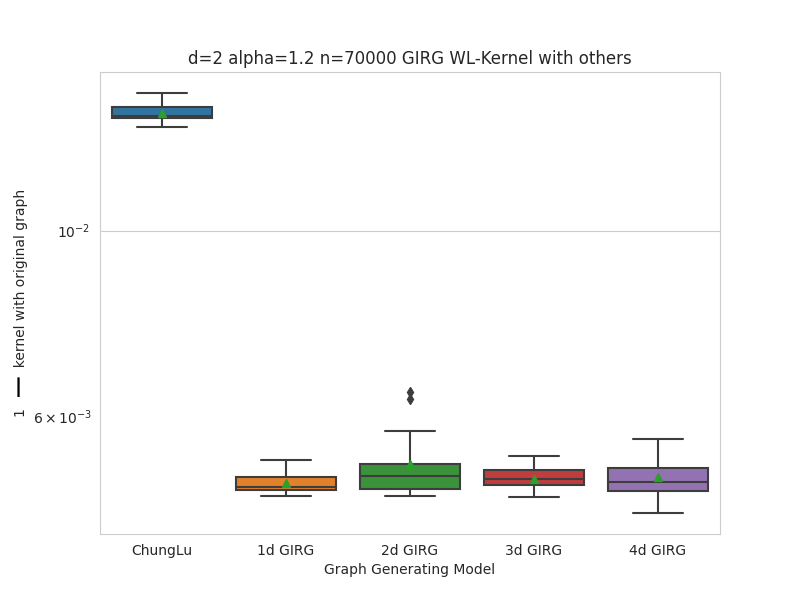
\includegraphics[width=0.8\linewidth]{figures/d=2 alpha=1.2 n=70000 GIRG WL-Kernel with others.png}
% \caption{WL-Kernel of a d=2, alpha=1.2, n=70000 Torus GIRG with other generated graphs (13 per model). All the GIRGs are more similar to the original than Chung-Lu, but we cannot differentiate between different GIRGs.}
% \label{fig:wl_kernel_gentorus}
% \end{figure}

% socfb-Brandeis99 d=3.png


% \begin{figure}
%   \centering
% 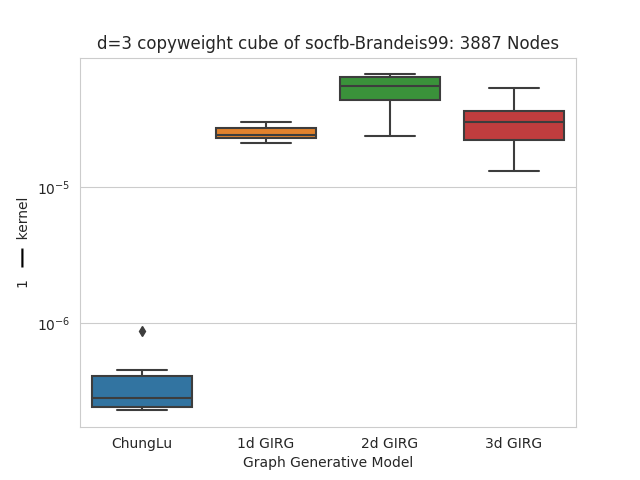
\includegraphics[width=0.8\linewidth]{figures/socfb-Brandeis99 d=3.png}
% \caption{RW-Kernel of a d=3 copy weight cube GIRG fit to socfb-Brandeis99 (matching number of edges and local clustering coefficient), with other generated graphs (6 per model type). Chung-Lu graphs have highest similarity to the original, despite it being a 3D GIRG}
% \label{fig:rw_kernel_fitcopycube}
% \end{figure}


